\documentclass[11pt,a4paper]{article}

% =====================================================================
% Packages
% =====================================================================

\usepackage[utf8]{inputenc}
\usepackage[T1]{fontenc}
\usepackage{lmodern}
\usepackage[english]{babel}
\usepackage{microtype}

\usepackage[
  left=2.6cm,
  right=2.6cm,
  top=2.5cm,
  bottom=2.5cm
]{geometry}

\usepackage{amsmath,amssymb,amsthm,mathtools}
\usepackage{bm}
\usepackage{booktabs}
\usepackage{array}
\usepackage{tabularx}
\usepackage{longtable}
\usepackage{enumitem}
\usepackage{graphicx}
\usepackage{xcolor}
\usepackage{url}
\usepackage[hidelinks]{hyperref}
\usepackage[nameinlink,noabbrev,capitalize]{cleveref}
\usepackage[round,authoryear]{natbib}
\usepackage{algorithm}
\usepackage{algpseudocode}
\usepackage{setspace}
\usepackage{caption}
\usepackage{subcaption}
\usepackage{tikz}
\usetikzlibrary{shapes,arrows.meta,positioning,fit,backgrounds,calc,chains,shadows}

\onehalfspacing

% =====================================================================
% General formatting
% =====================================================================

\setlength{\parindent}{0pt}
\setlength{\parskip}{5pt}

\setlist[itemize]{topsep=3pt,itemsep=2pt}
\setlist[enumerate]{topsep=3pt,itemsep=2pt}

\renewcommand{\arraystretch}{1.15}

% =====================================================================
% Mathematical environments
% =====================================================================

\newtheorem{definition}{Definition}
\newtheorem{assumption}{Assumption}
\newtheorem{theorem}{Theorem}
\newtheorem{proposition}{Proposition}
\newtheorem{lemma}{Lemma}
\newtheorem{corollary}{Corollary}
\newtheorem{remark}{Remark}

% =====================================================================
% Commands
% =====================================================================

\newcommand{\R}{\mathbb{R}}
\newcommand{\E}{\mathbb{E}}
\newcommand{\Prob}{\mathbb{P}}
\newcommand{\CVaR}{\operatorname{CVaR}}
\newcommand{\VaR}{\operatorname{VaR}}
\newcommand{\argmin}{\operatorname*{arg\,min}}
\newcommand{\cD}{\,{}^{C}\!D}
\newcommand{\OmegaM}{\Omega_M}
\newcommand{\dd}{\,\mathrm{d}}
\newcommand{\ind}{\mathbb{I}}

% =====================================================================
% Title and authors
% =====================================================================

\title{A Multistage Stochastic Transportation Model with
Caputo-Type Congestion Memory, Demand Uncertainty, and Carbon Trading}

\author{
Thiziri Sifaoui\textsuperscript{1}
\and
Madani Bezoui\textsuperscript{2,*}
\and
Meziane A{\"i}der\textsuperscript{3}
}

\date{}

\linespread{0.98}\selectfont
\begin{document}

\maketitle

\begin{center}
\small
\textsuperscript{1}
Department of Mathematics and Computer Science,
Faculty of Sciences and Technology,
University of Tamanrasset, Algeria\\
\texttt{t.sifaoui@univ-tamanrasset.dz}

\medskip

\textsuperscript{2}
CESI LINEACT, CESI Graduate School of Engineering,
2 All\'{e}e des Grandes Vignes, 54600 Villers-l\`{e}s-Nancy, France\\
\texttt{mbezoui@cesi.fr}

\medskip

\textsuperscript{3}
LaROMaD Laboratory, Faculty of Mathematics,
USTHB, Algiers, Algeria\\
\texttt{m-aider@usthb.dz}

\medskip

\ensuremath{^{\ast}}Corresponding author
\end{center}

% =====================================================================
% Abstract
% =====================================================================

\begin{abstract}
This paper introduces a multistage stochastic transportation model that
rigorously separates physical inventory conservation from hereditary
operational persistence. Physical usable inventory is governed by a
standard material-balance equation with proportional deterioration,
while an auxiliary fractional congestion state---governed by a Caputo-type
equation---captures persistent inbound-handling congestion. Demand
uncertainty is represented by a finite scenario tree in which continuous
sample paths are quantized into discrete nodal demand representatives,
and nodal non-anticipativity constraints ensure that operational
decisions depend only on information available at the corresponding
decision epoch. The formulation incorporates explicit lost sales,
transportation-mode activation, period-dependent carbon allowances,
endogenous allowance trading, cumulative service-level guarantees, and a
normalized convex combination of expected cost and Conditional
Value-at-Risk.

To ensure mathematical well-posedness across the entire parameter
domain, the Caputo operator is discretized via a piecewise L1 formula
that explicitly defines the first-order limit without encountering
undefined exponential expressions. The memory modulation constraint is
formulated using only the beginning-of-period memory state and is
linearized exactly into a pair of affine inequalities, preserving the
mixed-integer linear structure. We prove positivity and decay of the
discrete weights, convergence of the discrete fractional operator to the
backward first-order difference as the fractional order approaches one,
finite-horizon input-to-state boundedness of the discrete memory state,
existence of an optimal policy under explicit boundedness assumptions,
and the existence of an optimal nodal trading policy without
simultaneous carbon-allowance buying and selling when the buying price
strictly exceeds the selling price.

A Sample Average Approximation and Progressive Hedging framework is
specified for computational implementation, with a probability-weighted
scenario decomposition that correctly reproduces the normalized
mean--CVaR objective. A supplementary computational archive accompanies the manuscript and contains the Python source code, generated scenario-tree instance, random seeds, raw Progressive Hedging histories, parameter-estimation profiles, and solver logs. A small synthetic study is reported as an implementation and reproducibility check; it is not intended as large-scale or empirical validation. Instead, it establishes a comprehensive
reproducibility and validation protocol covering parameter
identification, scenario-tree reduction error, deterministic-equivalent
benchmarks, repeated-sample assessment, out-of-sample evaluation, and
mixed-integer Progressive Hedging validation.
\end{abstract}

\noindent
\textbf{Keywords:}
fractional optimization,
Caputo derivative,
multistage stochastic programming,
transportation planning,
carbon trading,
Conditional Value-at-Risk,
Sample Average Approximation,
Progressive Hedging,
non-anticipativity.

% =====================================================================
\section{Introduction}
% =====================================================================

Transportation and distribution systems must simultaneously address
economic efficiency, service continuity, uncertain demand, and
environmental regulation. Standard multi-period transportation models
usually represent operational states through first-order recursions. Such
recursions are appropriate when the state at one period summarizes all
relevant information from the past. They can, however, be restrictive
when operational effects persist over several periods.

Examples of persistent effects include repeated handling losses, gradual
deterioration, and long-lasting capacity degradation. Fractional
calculus provides one possible phenomenological representation of such
persistence \citep{caputo1967,podlubny1999,diethelm2010}. In particular,
a Caputo derivative depends on the complete history of state increments
through a power-law kernel.

The use of a fractional operator does not, by itself, prove that a
transportation system possesses fractional dynamics. Furthermore, a
physical inventory state must rigorously obey a material conservation
law. This paper therefore distinguishes physical usable inventory---which
follows an ordinary conservation equation---from an auxiliary fractional
state representing \emph{persistent inbound-handling congestion}. Positive
values of this memory state arise when delivered volume exceeds fulfilled
demand, and they reduce future fulfillment capacity. Negative values
represent handling slack or recovery capacity; they do not directly
increase fulfillment beyond the physical-stock bound, but they can
partially offset subsequent positive congestion through the memory
dynamics.

Uncertainty is another essential component of transportation planning.
Multistage stochastic programming provides a framework in which each
decision depends only on observations available at its decision epoch
\citep{birge2011,shapiro2014}. This information structure is more
appropriate than a two-stage representation when shipments are revised
sequentially and future demand is not revealed at the beginning of the
planning horizon.

Environmental regulation is represented through period-dependent
carbon allowances and allowance trading. Unlike a fixed emissions tax,
a cap-and-trade mechanism permits the planner to purchase additional
allowances or sell unused allowances. Related sustainable
transportation and supply-chain models demonstrate the importance of
jointly considering operational costs and emissions
\citep{bektas2011pollution,asghari2021green,qu2021carbon,mirzaee2024green,gbadegoye2025intermodal}.

Risk aversion is represented by Conditional Value-at-Risk (CVaR).
CVaR is suitable for this purpose because it penalizes the severity of
high-cost outcomes and possesses a tractable optimization
representation \citep{rockafellar2000,rockafellar2002cvar}. We explicitly
note that while the operational policy is multistage and non-anticipative,
the risk measure is a static ex-ante CVaR evaluated over the total-horizon
cost. Although this captures terminal tail risk without requiring nested
conditional risk mappings, static ex-ante risk measures may exhibit
temporal inconsistency across intermediate decision stages.

The contributions of this paper are as follows.

\begin{enumerate}
  \item We formulate a multistage stochastic transportation model that
  rigorously separates physical usable inventory from an auxiliary
  fractional inbound-handling congestion state, incorporating explicit
  lost sales and cumulative service requirements.

  \item We define a piecewise L1 discrete operator for the Caputo equation
  that remains well-defined over the full domain \(\alpha\in(0,1]\) and
  recovers the ordinary first-order difference at \(\alpha=1\).

  \item We specify a scenario-tree construction procedure based on
  conditional distance clustering that quantizes continuous sample
  paths into discrete nodal demand representatives, preventing
  non-anticipativity from collapsing into artificial perfect information.

  \item We derive a finite-dimensional deterministic equivalent under a
  normalized convex mean--CVaR objective, establish analytical
  properties including nodal carbon-trading separation, and prove
  finite-horizon input-to-state boundedness of the discrete memory
  state.

  \item We specify a probability-weighted SAA--Progressive Hedging
  architecture that correctly decomposes the normalized mean--CVaR
  objective, without claiming global convergence for the mixed-integer
  case.

  \item We provide a reproducible experimental protocol while excluding
  numerical results that are not supported by verifiable data, code,
  solver logs, and scenario-level outputs.
\end{enumerate}

The remainder of the paper is organized as follows.
\Cref{sec:literature} reviews the related literature.
\Cref{sec:preliminaries} introduces the fractional and stochastic
concepts.
\Cref{sec:assumptions} states the modeling and dimensional assumptions.
\Cref{sec:model} presents the multistage model.
\Cref{sec:properties} establishes its analytical properties.
\Cref{sec:solution} describes the computational methodology.
\Cref{sec:protocol} gives the validation protocol.
\Cref{sec:managerial} discusses managerial interpretation.
\Cref{sec:limitations} discusses limitations, and
\Cref{sec:conclusion} concludes.

% =====================================================================
\section{Related Literature}
\label{sec:literature}
% =====================================================================

\subsection{Stochastic transportation planning}

Stochastic programming distinguishes decisions made before uncertainty
is observed from decisions made after additional information becomes
available. Two-stage models assume that the complete uncertain outcome
is revealed between the first and second stages. Multistage models
instead represent sequential information revelation
\citep{birge2011,shapiro2014}.

This distinction is important in transportation planning. If shipments
are selected period by period, a decision at period \(t\) should not
depend on demands observed only after period \(t\). The present paper
therefore uses scenario histories and explicit non-anticipativity
constraints.

Recent transportation models combine uncertain demand, capacity,
emissions, and risk measures. For example,
\citet{gbadegoye2025intermodal} consider road--rail intermodal
transportation under demand and capacity uncertainty. The present
formulation differs by introducing an auxiliary fractional memory state
and period-adapted carbon trading.

\subsection{Sustainable transportation and carbon regulation}

The pollution-routing problem demonstrates that transportation costs
and emissions can lead to structurally different routing decisions
\citep{bektas2011pollution}. The broader green vehicle-routing
literature confirms that emissions depend on operational decisions and
cannot always be treated as a fixed post-processing measure
\citep{asghari2021green}.

Robust and stochastic supply-chain models have also incorporated carbon
regulation and disruption risk
\citep{qu2021carbon,mirzaee2024green}. The present paper treats
allowance purchases and sales as adaptive decisions. To avoid an
unbounded trading representation, both variables have explicit finite
bounds.

\subsection{Fractional dynamics}

Fractional derivatives provide a nonlocal representation of dynamics
with hereditary effects \citep{caputo1967,podlubny1999,diethelm2010}.
The Caputo derivative is especially convenient when initial conditions
are expressed using the state itself.

The L1 formula is a standard discretization of the Caputo derivative.
Its coefficients are positive and decreasing, and it creates coupling
between each period and all previous state increments
\citep{lin2007}. Faster approximations can become useful for long
horizons \citep{zhang2022fast}.

Fractional ideas have also appeared in inventory and supply-chain
applications \citep{cuong2023,haque2026}. Nevertheless, the use of a
fractional operator in optimization requires particular care. A
physical inventory must respect mass conservation; fractional equations
should therefore govern auxiliary memory or degradation states whose
parameters must be calibrated jointly from empirical data.

\subsection{Scenario-tree construction}

Representing a continuous stochastic process by a finite scenario tree
requires careful discretization to preserve the information structure.
\citet{dupacova2003scenarios} introduce scenario reduction via
probability metrics, establishing that a reduced tree can approximate
the original distribution. For multistage processes, tree quality must
be evaluated using a filtration-aware metric such as the nested distance
\citep{pflug2012distance}.
\citet{heitsch2009scenario} extend this framework to multistage trees,
providing algorithms for stagewise scenario reduction that preserve
temporal dependence. These references motivate the scenario-tree
construction protocol proposed for future implementation in this paper.

\subsection{CVaR, SAA, and Progressive Hedging}

The Rockafellar--Uryasev representation expresses CVaR through a scalar
threshold and nonnegative excess variables
\citep{rockafellar2000,rockafellar2002cvar}. This representation is
compatible with finite-scenario stochastic optimization.

Sample Average Approximation replaces an expectation with an empirical
average computed from sampled scenarios. Its reliability must be
assessed through independent testing and repeated samples
\citep{kleywegt2002saa,shapiro2014}. Randomized quasi-Monte Carlo
sampling may also improve estimation in suitable risk-averse problems
\citep{melnikov2025rqmc}.

Progressive Hedging decomposes a scenario problem by temporarily
relaxing non-anticipativity and penalizing disagreement between scenario
copies \citep{rockafellar1991}. Its classical convergence theory is
based on convexity. In stochastic integer programming, it is commonly
used as a heuristic, and its output must be validated against
deterministic-equivalent solutions whenever possible
\citep{christiansen2023ph}.

% =====================================================================
\section{Fractional and Stochastic Preliminaries}
\label{sec:preliminaries}
\label{sec:preliminaries}
% =====================================================================

\subsection{Caputo derivative}

\begin{definition}[Caputo derivative]
Let \(w:[0,\tau_N]\rightarrow\R\) be absolutely continuous and let
\(0<\alpha<1\). The Caputo derivative of order \(\alpha\) is
\begin{equation}
  \cD_{\tau}^{\alpha}w(\tau)
  =
  \frac{1}{\Gamma(1-\alpha)}
  \int_{0}^{\tau}
  \frac{w'(s)}{(\tau-s)^{\alpha}}
  \dd s.
  \label{eq:caputo}
\end{equation}
\end{definition}

The kernel in \cref{eq:caputo} gives nonzero weight to the full
trajectory of past increments. The fractional order controls the
decay pattern but should not be interpreted independently from the
other dynamic parameters.

\subsection{Normalized time and units}

Let \(t_{\mathrm{ref}}>0\) be a reference time and define
\[
  \tau=\frac{t_{\mathrm{physical}}}{t_{\mathrm{ref}}}.
\]
The normalized time \(\tau\) is dimensionless. Therefore,
\(\cD_{\tau}^{\alpha}w\) has the same physical unit as \(w\).

If the fractional equation is written in physical time instead, then
\[
  \cD_{\tau}^{\alpha}w
  =
  t_{\mathrm{ref}}^{\alpha}
  \cD_{t_{\mathrm{physical}}}^{\alpha}w.
\]
The reference-time factor must consequently be retained when parameters
are transferred between time scales.

\subsection{Piecewise L1 discretization}
\label{sec:piecewise-l1}

Consider a uniform normalized grid \(\tau_t=t\Delta\tau\) for
\(t=0,\ldots,N\). For \(0<\alpha<1\), define the weights
\begin{equation}
  a_{\ell}^{(\alpha)}
  =
  (\ell+1)^{1-\alpha}-\ell^{1-\alpha},
  \qquad
  \ell=0,\ldots,N-1.
  \label{eq:l1weights}
\end{equation}
To ensure that the discrete fractional operator remains formally defined
over the entire domain \(\alpha\in(0,1]\) without generating undefined
expressions of the form \(0^{0}\) at \(\alpha=1\), we define the piecewise
discrete operator:
\begin{equation}
  \mathcal{D}_{\Delta\tau}^{\alpha}w_t
  =
  \begin{cases}
    \displaystyle
    \frac{1}{
      \Gamma(2-\alpha)(\Delta\tau)^\alpha
    }
    \sum_{\ell=0}^{t-1}
    a_{t-\ell-1}^{(\alpha)}
    \left(w_{\ell+1}-w_\ell\right),
    & 0<\alpha<1,\\[3ex]
    \displaystyle
    \frac{w_t-w_{t-1}}{\Delta\tau},
    & \alpha=1.
  \end{cases}
  \label{eq:discrete-operator}
\end{equation}
Because \(\Delta\tau\) is dimensionless, \(\mathcal{D}_{\Delta\tau}^{\alpha}w_t\)
has the same physical unit as \(w_t\). When \(\alpha=1\), this operator
directly recovers the backward first-order difference.

\subsection{Scenario-tree construction via nodal quantization}

\begin{figure}[h]
    \centering
    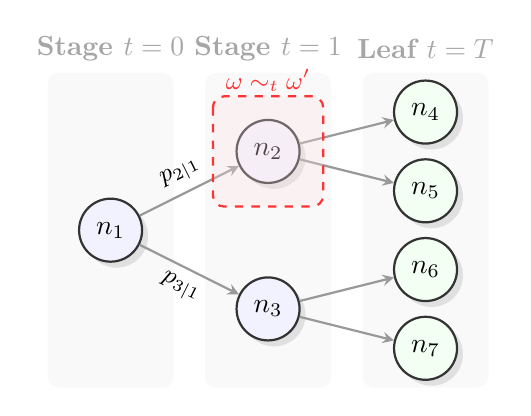
\begin{tikzpicture}[
        node distance=1.5cm and 2cm,
        cnode/.style={circle, draw=black!80, fill=blue!5, thick, minimum size=8mm, drop shadow={opacity=0.2}},
        leaf/.style={circle, draw=black!80, fill=green!5, thick, minimum size=8mm, drop shadow={opacity=0.2}},
        branch/.style={->, thick, >=stealth, draw=gray!80}
    ]
        % Background Stages
        \begin{scope}[on background layer]
            \fill[gray!5, rounded corners] (-0.8, 2) rectangle (0.8, -2);
            \node[gray!70, font=\bfseries] at (0, 2.3) {Stage $t=0$};
            
            \fill[gray!5, rounded corners] (1.2, 2) rectangle (2.8, -2);
            \node[gray!70, font=\bfseries] at (2, 2.3) {Stage $t=1$};

            \fill[gray!5, rounded corners] (3.2, 2) rectangle (4.8, -2);
            \node[gray!70, font=\bfseries] at (4, 2.3) {Leaf $t=T$};
        \end{scope}

        % Nodes
        \node[cnode] (n1) at (0, 0) {$n_1$};
        \node[cnode] (n2) at (2, 1) {$n_2$};
        \node[cnode] (n3) at (2, -1) {$n_3$};
        \node[leaf] (n4) at (4, 1.5) {$n_4$};
        \node[leaf] (n5) at (4, 0.5) {$n_5$};
        \node[leaf] (n6) at (4, -0.5) {$n_6$};
        \node[leaf] (n7) at (4, -1.5) {$n_7$};

        % Edges
        \draw[branch] (n1) -- (n2) node[midway, above, sloped, font=\small, text=black] {$p_{2|1}$};
        \draw[branch] (n1) -- (n3) node[midway, below, sloped, font=\small, text=black] {$p_{3|1}$};
        \draw[branch] (n2) -- (n4);
        \draw[branch] (n2) -- (n5);
        \draw[branch] (n3) -- (n6);
        \draw[branch] (n3) -- (n7);

        % Non-anticipativity grouping (example)
        \draw[dashed, red!80, thick, rounded corners, fill=red!10, fill opacity=0.3] (1.3, 1.7) rectangle (2.7, 0.3);
        \node[red!80, font=\small\bfseries] at (2, 1.9) {$\omega \sim_{t} \omega'$};
    \end{tikzpicture}
    \caption{Stochastic information structure represented as a discrete scenario tree. Non-anticipativity conditions are enforced at nodes shared by multiple scenarios.}
    \label{fig:scenario_tree_tikz}
\end{figure}
\label{sec:tree-construction}

When underlying demand uncertainty originates from continuous stochastic
processes (such as drift-diffusion), continuous sample paths almost surely
differ at every decision epoch (\(d_{j1}^{\omega}\neq d_{j1}^{\omega'}\)).
Defining information equivalence by exact equality of continuous trajectories
would collapse non-anticipativity into artificial perfect information, as
every scenario would branch into its own node at period~1.

To prevent this, scenario histories must be constructed through a formal
discretization and tree-reduction procedure
\citep{dupacova2003scenarios,heitsch2009scenario}. The procedure operates as
follows.

\begin{enumerate}
  \item \textbf{Sample generation.} Generate a large ensemble of
  \(M_0\gg|\Omega|\) continuous demand trajectories from the underlying
  stochastic model.

  \item \textbf{Stagewise conditional clustering.} At each period \(t\),
  partition the trajectories passing through each parent node
  \(n\in\mathcal{N}_{t-1}\) into \(B_t(n)\) child clusters. Candidate
  reduced trees are evaluated using a filtration-aware metric,
  preferably nested distance.

  \item \textbf{Nodal demand quantization.} Each cluster at period \(t\)
  defines a unique node \(n\in\mathcal{N}_t\) with a representative demand
  vector \(\widehat{d}_{jtn}\). All scenarios passing through node \(n\) use
  this same representative demand at period \(t\):
  \begin{equation}
    d_{jt}^{\omega}
    =
    \widehat{d}_{jtn}
    \qquad
    \text{whenever }n_t(\omega)=n.
    \label{eq:nodal-demand}
  \end{equation}
  Consequently, scenarios sharing a node are observationally
  indistinguishable, and their demand-balance and non-anticipativity
  constraints remain compatible.

  \item \textbf{Conditional probabilities.} The probability of node \(n\)
  conditional on its parent is derived from cluster frequencies.

  \item \textbf{Tree-reduction error.} Tree quality must be evaluated
  using a filtration-aware probability metric. Preferably, the nested
  distance between the original sampled process and the reduced scenario
  tree should be reported. When an ordinary Wasserstein metric is used
  as a computational approximation, this limitation must be stated
  explicitly.
\end{enumerate}

Define \(\Omega(n) = \{\omega\in\Omega:n_t(\omega)=n\}\). Let \(\Omega\) be the resulting finite set of complete scenario paths with
probabilities \(p_\omega>0\), where \(\sum_{\omega\in\Omega}p_\omega=1\).
The information equivalence relation is defined nodally:
\begin{equation}
  \omega\sim_t\omega'
  \quad\Longleftrightarrow\quad
  n_t(\omega)=n_t(\omega').
  \label{eq:history-equivalence}
\end{equation}
Decisions at period \(t\) must be identical for all scenarios sharing the
same history node under \(\sim_t\).

\subsection{Conditional Value-at-Risk}

For a finite-scenario cost \(C^\omega\), CVaR at confidence level
\(\beta\in(0,1)\) is represented by
\begin{equation}
  \CVaR_\beta(C)
  =
  \min_{\eta\in\R}
  \left\{
    \eta
    +
    \frac{1}{1-\beta}
    \sum_{\omega\in\Omega}
    p_\omega
    \left(C^\omega-\eta\right)_+
  \right\}.
  \label{eq:cvar-definition}
\end{equation}
Introducing \(\xi^\omega\geq0\) gives the linear inequalities:
\begin{equation}
  \xi^\omega\geq C^\omega-\eta,
  \qquad
  \xi^\omega\geq0.
  \label{eq:cvar-linearization}
\end{equation}

% =====================================================================
\section{Multistage Model}
\label{sec:model}

\subsection{Ex-ante bounds on operational dynamics}
To ensure computational tractability and numerical stability for the fractional memory state, we explicitly bound the realized deliveries and demand using:
\[
\overline d_{jt}
=
\max_{n\in\mathcal N_t}\widehat d_{jtn},
\]
\[
\overline r_{jt}
=
\min
\left\{
\sum_{i\in I}S_{it},
\sum_{k\in K}Q_{kt}
\right\}.
\]
Consequently, the fractional forcing sequence is strictly bounded by:
\[
|F_t^\omega|
\le
\psi_j
\left(
\overline r_{jt}+\overline d_{jt}
\right).
\]

\subsection{Modeling assumptions and dimensional conventions}
\label{sec:assumptions}
% =====================================================================

\begin{assumption}[State distinction]
\label{ass:state}
The variable \(z_{jt}^{\omega}\) denotes the physical usable inventory of
customer \(j\) at the end of period \(t\) under scenario \(\omega\), governed
by an ordinary material conservation law. A distinct state variable \(m_{jt}^{\omega}\) represents an auxiliary
Caputo-type congestion-memory state capturing persistent inbound-handling congestion
generated when delivered volume exceeds fulfilled demand. Positive values
of \(m_{jt}^{\omega}\) reduce effective fulfillment capacity. Negative values of the memory state
represent handling slack; they do not directly increase fulfillment
but can partially offset subsequent congestion.
\end{assumption}

\begin{assumption}[Chronological sequence and demand timing]
\label{ass:chronology}
Within each decision epoch \(t\) and history node \(n_t(\omega)\), events
follow a strict chronological order:
\begin{enumerate}[label=(\roman*)]
  \item observation of the nodal demand representative
  \(\widehat{d}_{jtn}\) defined in \cref{eq:nodal-demand};
  \item observation of beginning-of-period states
  \(z_{j,t-1}^{\omega}\) and \(m_{j,t-1}^{\omega}\);
  \item determination of operational delivery
  \(x_{ijkt}^{\omega}\), fulfilled demand \(q_{jt}^{\omega}\), and
  lost sales \(u_{jt}^{\omega}\);
  \item evaluation of period carbon emissions \(E_t^\omega\);
  \item selection of allowance purchases \(b_t^\omega\) and sales
  \(s_t^\omega\), modeled as an end-of-period compliance decision
  where realized operational emissions are known before trading;
  \item update of physical inventory \(z_{jt}^{\omega}\) and memory
  state \(m_{jt}^{\omega}\).
\end{enumerate}
Consequently, fulfillment decisions depend on \(m_{j,t-1}^{\omega}\)
(known at step~(ii)), not on \(m_{jt}^{\omega}\) (computed at
step~(vi)).
\end{assumption}

\begin{assumption}[Negligible lead time]
\label{ass:leadtime}
Transportation lead times are assumed negligible relative to the length
of one planning period. Hence \(x_{ijkt}^{\omega}\) denotes both the
quantity dispatched and delivered during period \(t\), and supplier
availability \(S_{it}\) applies at the same period.
\end{assumption}

\begin{assumption}[Lost sales]
\label{ass:lostsales}
Unfulfilled demand is lost rather than backlogged. A model with backlog
would require a separate state variable and a different interperiod balance.
\end{assumption}

\begin{assumption}[Fractional interpretation]
\label{ass:fractional}
The fractional equation governing \(m_{jt}^{\omega}\) is a phenomenological
constitutive model for inbound-handling congestion. The memory coupling
coefficient \(\psi_j\), fractional order \(\alpha\), and dissipation
coefficient \(\rho_j\) must be estimated jointly from empirical
observations. The operational interpretation is as follows: positive
values of \(m_{jt}^{\omega}\) represent persistent inbound-handling
congestion generated when delivered volume exceeds fulfilled demand;
negative values represent handling slack; they do not directly
increase fulfillment beyond the physical inventory limit but can offset
future congestion.
\end{assumption}

\begin{assumption}[Bounded planning domain]
\label{ass:bounds}
Supply, transportation capacity, demand, usable inventory, memory states,
carbon trading, and all cost coefficients are finite. The feasible set is
assumed nonempty. \Cref{tab:dimensions} summarizes the dimensional
conventions and physical units used throughout this paper.
\end{assumption}

\begin{table}[htbp]
\centering
\renewcommand{\arraystretch}{1.25}
\caption{Dimensional conventions and physical units.}
\label{tab:dimensions}
\begin{tabularx}{\textwidth}{@{}lllX@{}}
\toprule
Symbol & Interpretation & Unit & Comment\\
\midrule
\(\tau\) & normalized time & dimensionless &
  \(\tau=t_{\mathrm{physical}}/t_{\mathrm{ref}}\)\\
\(z\) & physical usable inventory & product &
  end-of-period physical stock\\
\(m\) & handling-congestion memory & product &
  L1-discretized persistent imbalance\\
\(x\) & dispatched and delivered quantity & product &
  negligible lead time assumed\\
\(q\) & fulfilled demand & product &
  quantity served within period \(\tau_t\)\\
\(u\) & lost sales & product &
  unfulfilled part of demand\\
\(\widehat{d}\) & nodal demand representative & product &
  \(\widehat{d}=q+u\) at each node\\
\(\delta\) & inventory deterioration & dimensionless &
  physical stock proportional loss\\
\(\psi\) & memory coupling coefficient & dimensionless &
  scales the net-imbalance forcing\\
\(\rho\) & memory dissipation factor & dimensionless &
  estimated jointly with \(\alpha\)\\
\(\chi\) & memory modulation coefficient & dimensionless &
  reduces fulfillment when \(m>0\)\\
\(e\) & emission factor & carbon/product &
  multiplied by delivered quantity\\
\(A,b,s\) & allowances and trades & carbon &
  period-dependent carbon quantities\\
\bottomrule
\end{tabularx}
\end{table}

% =====================================================================
\subsection{Multistage stochastic transportation model}
\label{sec:model}
% =====================================================================

\subsection{Sets and indices}

\begin{itemize}
  \item \(I\): suppliers, indexed by \(i\);
  \item \(J\): customers, indexed by \(j\);
  \item \(K\): transportation modes, indexed by \(k\);
  \item \(T=\{1,\ldots,N\}\): planning periods, indexed by \(t\);
  \item \(\Omega\): scenario paths in the discrete tree,
  indexed by~\(\omega\);
  \item \(\mathcal{N}_t\): set of history nodes at period \(t\).
\end{itemize}

\subsection{Parameters}

\begin{itemize}
  \item \(p_\omega>0\): probability of scenario \(\omega\);
  \item \(S_{it}\geq0\): supply available from supplier \(i\) in
  period~\(t\);
  \item \(\widehat{d}_{jtn}\geq0\): nodal demand representative for
  customer \(j\) at node \(n\in\mathcal{N}_t\);
  \item \(c_{ijkt}\geq0\): unit shipment cost;
  \item \(f_k\geq0\): fixed activation cost of mode \(k\);
  \item \(Q_{kt}\geq0\): period capacity of mode \(k\);
  \item \(h_{jt}\geq0\): physical inventory holding cost;
  \item \(\pi_{jt}\geq0\): lost-sales penalty;
  \item \(e_{ijkt}\geq0\): unit carbon emissions;
  \item \(A_t\geq0\): initial carbon allowance for period \(t\);
  \item \(p_t^b>p_t^s\geq0\): allowance buying and selling prices;
  \item \(\overline{B}_t<\infty\): upper bound on allowance purchases;
  \item \(\overline{S}_t<\infty\): upper bound on allowance sales;
  \item \(z_j^0\geq0\): initial physical usable inventory;
  \item \(\overline{z}_{jt}<\infty\): physical inventory capacity;
  \item \(\delta_j\in[0,1)\): physical inventory deterioration
  coefficient;
  \item \(\psi_j>0\): dimensionless memory coupling coefficient;
  \item \(\rho_j\geq0\): normalized memory dissipation coefficient;
  \item \(\chi_j (calibrated separately from observations linking beginning-of-period congestion to reductions in effective fulfillment capacity)\in[0,1)\): memory modulation coefficient on
  fulfillment;
  \item \(\overline{m}_{jt}<\infty\): upper bound on absolute memory
  state;
  \item \(\gamma_j\in[0,1]\): minimum cumulative service fraction;
  \item \(\alpha\in(0,1]\): fractional order;
  \item \(\beta\in(0,1)\): CVaR confidence level;
  \item \(\lambda\in[0,1]\): normalized weight of the CVaR term;
  \item \(\Delta\tau>0\): normalized grid spacing.
\end{itemize}

\subsection{Decision variables}

The strategic decision is \(y_k\in\{0,1\}\), where \(y_k=1\) if mode \(k\)
is activated. For each scenario \(\omega\) and period \(t\), define:
\begin{align*}
  x_{ijkt}^{\omega}&\geq0 &&\text{quantity dispatched and delivered
  from \(i\) to \(j\) via \(k\)},\\
  q_{jt}^{\omega}&\geq0 &&\text{fulfilled demand},\\
  u_{jt}^{\omega}&\geq0 &&\text{lost sales},\\
  z_{jt}^{\omega}&\geq0 &&\text{physical usable inventory},\\
  m_{jt}^{\omega}&\in\R &&\text{inbound-handling congestion memory},\\
  b_t^\omega&\geq0 &&\text{allowances purchased},\\
  s_t^\omega&\geq0 &&\text{allowances sold}.
\end{align*}
The CVaR variables are \(\eta\in\R\) and \(\xi^\omega\geq0\).

\subsection{Scenario cost}

The adaptive operating cost under scenario \(\omega\) is
\begin{align}
  C^\omega
  ={}&
  \sum_{t\in T}
  \sum_{i\in I}
  \sum_{j\in J}
  \sum_{k\in K}
  c_{ijkt}x_{ijkt}^{\omega}
  +
  \sum_{t\in T}
  \sum_{j\in J}
  \left(
    h_{jt}z_{jt}^{\omega}
    +
    \pi_{jt}u_{jt}^{\omega}
  \right)
  \nonumber\\
  &+
  \sum_{t\in T}
  \left(
    p_t^b b_t^\omega
    -
    p_t^s s_t^\omega
  \right).
  \label{eq:scenario-cost}
\end{align}
The fixed activation cost is kept outside \(C^\omega\) because it is
identical in every scenario.

\subsection{Objective function}

To avoid unnormalized double counting of operating costs and make the
risk preference transparent, we adopt a normalized convex combination
of expected cost and CVaR:
\begin{equation}
\begin{aligned}
  \min\quad
  &
  \sum_{k\in K}f_ky_k
  +
  (1-\lambda)
  \sum_{\omega\in\Omega}p_\omega C^\omega
  \\
  &+
  \lambda
  \left[
    \eta
    +
    \frac{1}{1-\beta}
    \sum_{\omega\in\Omega}p_\omega\xi^\omega
  \right],
\end{aligned}
\label{eq:objective}
\end{equation}
where \(\lambda\in[0,1]\). Here, \(\lambda=0\) represents pure
risk-neutral expectation minimization, whereas \(\lambda=1\) represents
pure CVaR minimization. Because the fixed activation cost is deterministic,
translation equivariance implies that if total cost is \(T=\sum_kf_ky_k+C\), then
\((1-\lambda)\mathbb{E}[T]+\lambda\CVaR_\beta(T) = \sum_k f_ky_k+(1-\lambda)\mathbb{E}[C]+\lambda\CVaR_\beta(C)\),
justifying the placement of the fixed cost outside the scenario-dependent term.

\subsection{Supply and mode capacity}

For all \(i\in I\), \(t\in T\), and \(\omega\in\Omega\),
\begin{equation}
  \sum_{j\in J}\sum_{k\in K}
  x_{ijkt}^{\omega}
  \leq S_{it}.
  \label{eq:supply}
\end{equation}
For all \(k\in K\), \(t\in T\), and \(\omega\in\Omega\),
\begin{equation}
  \sum_{i\in I}\sum_{j\in J}
  x_{ijkt}^{\omega}
  \leq Q_{kt}y_k.
  \label{eq:mode-capacity}
\end{equation}

\subsection{Demand fulfillment, lost sales, and cumulative service}

Because each scenario \(\omega\) passing through node
\(n=n_t(\omega)\) uses the common representative demand
\(\widehat{d}_{jtn}\), the demand split is written for all
\(j\in J\), \(t\in T\), and \(\omega\in\Omega\):
\begin{equation}
  q_{jt}^{\omega}+u_{jt}^{\omega}
  =
  \widehat{d}_{jt,n_t(\omega)},
  \label{eq:demand-split}
\end{equation}
with
\begin{equation}
  0\leq q_{jt}^{\omega}\leq \widehat{d}_{jt,n_t(\omega)},
  \qquad
  0\leq u_{jt}^{\omega}\leq \widehat{d}_{jt,n_t(\omega)}.
  \label{eq:demand-bounds}
\end{equation}
To ensure that service continuity is maintained throughout the horizon
rather than compensated only at the end, we impose a cumulative service
requirement:
\begin{equation}
  \sum_{\tau=1}^{t}q_{j\tau}^{\omega}
  \geq
  \gamma_j
  \sum_{\tau=1}^{t}\widehat{d}_{j\tau,n_\tau(\omega)},
  \qquad
  j\in J,\ t\in T,\ \omega\in\Omega.
  \label{eq:service}
\end{equation}
\Cref{eq:service} can make some scenarios infeasible; feasibility must
therefore be checked for every generated instance.

\subsection{Initial conditions}

For every \(j\in J\) and \(\omega\in\Omega\),
\begin{equation}
  z_{j0}^{\omega}=z_j^0,
  \qquad
  m_{j0}^{\omega}=0.
  \label{eq:initial-condition}
\end{equation}
Initial values are common across scenarios because no uncertainty has
been observed before the planning horizon.

\subsection{Physical inventory balance and fractional memory state}

\begin{figure}[h]
    \centering
    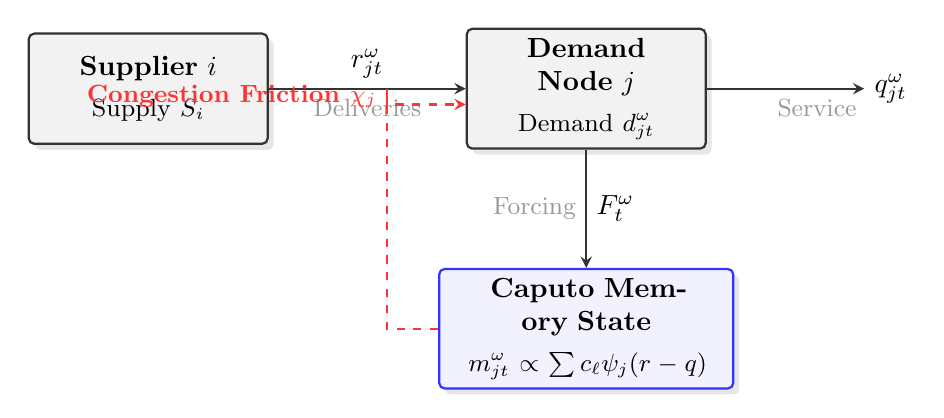
\begin{tikzpicture}[
        node distance=2.5cm,
        box/.style={rectangle, draw=black!80, thick, fill=gray!10, text width=2.8cm, align=center, minimum height=1.4cm, drop shadow={opacity=0.2}, rounded corners=2pt},
        membox/.style={rectangle, draw=blue!80, thick, fill=blue!5, text width=3.5cm, align=center, minimum height=1.4cm, drop shadow={opacity=0.2}, rounded corners=2pt},
        arrow/.style={->, thick, >=stealth, draw=black!80}
    ]
        % Nodes
        \node[box] (supply) {\textbf{Supplier $i$}\\[1mm] \small Supply $S_i$};
        \node[box, right=of supply] (nodej) {\textbf{Demand Node $j$}\\[1mm] \small Demand $d_{jt}^\omega$};
        \node[membox, below=1.5cm of nodej] (memory) {\textbf{Caputo Memory State}\\[1mm] \small $m_{jt}^\omega \propto \sum c_\ell \psi_j (r-q)$};
        
        % Paths
        \draw[arrow] (supply) -- (nodej) node[midway, above, font=\bfseries] {$r_{jt}^\omega$} node[midway, below, font=\small, text=gray!80] {Deliveries};
        \draw[arrow] (nodej.east) -- +(2,0) node[right, font=\bfseries] {$q_{jt}^\omega$} node[pos=0.7, below, font=\small, text=gray!80] {Service};
        \draw[arrow] (nodej.south) -- (memory.north) node[midway, right, font=\bfseries] {$F_t^\omega$} node[midway, left, font=\small, text=gray!80] {Forcing};
        \draw[arrow, dashed, draw=red!80, thick] (memory.west) -| ([xshift=-1cm]nodej.west) |- ([yshift=-2mm]nodej.west) node[pos=0.25, left, font=\small\bfseries, text=red!80] {Congestion Friction $\chi_j$};
    \end{tikzpicture}
    \caption{Coupled dynamics of physical inventory delivery and the fractional congestion memory state.}
    \label{fig:physical_fractional_diagram}
\end{figure}
Let \(r_{jt}^{\omega}=\sum_{i\in I}\sum_{k\in K}x_{ijkt}^{\omega}\) be
the total quantity delivered to customer \(j\) during period \(t\).

The physical usable inventory strictly respects material conservation
with proportional deterioration \(\delta_j\in[0,1)\):
\begin{equation}
  z_{jt}^{\omega}
  =
  (1-\delta_j)z_{j,t-1}^{\omega}
  +
  r_{jt}^{\omega}
  -
  q_{jt}^{\omega},
  \qquad
  0\leq z_{jt}^{\omega}\leq\overline{z}_{jt}.
  \label{eq:physical-balance}
\end{equation}

To capture persistent inbound-handling congestion, the auxiliary memory
state \(m_{jt}^{\omega}\) is governed by the piecewise discrete operator
defined in \cref{eq:discrete-operator}:
\begin{equation}
  \mathcal{D}_{\Delta\tau}^{\alpha}m_{jt}^{\omega}
  =
  \psi_j\left(r_{jt}^{\omega}-q_{jt}^{\omega}\right)
  -
  \rho_jm_{jt}^{\omega},
  \qquad
  -\overline{m}_{jt}\leq m_{jt}^{\omega}\leq\overline{m}_{jt}.
  \label{eq:discrete-fractional-balance}
\end{equation}

The memory state modulates operational fulfillment capacity using the
beginning-of-period memory \(m_{j,t-1}^{\omega}\), which is known before
any period-\(t\) decision is taken (see
\cref{ass:chronology}, step~(ii)). This avoids instantaneous algebraic
feedback between \(q_{jt}^{\omega}\) and \(m_{jt}^{\omega}\). The
resulting constraint is linearized exactly into the following pair of
affine inequalities:
\begin{subequations}
\label{eq:memory-modulation}
\begin{align}
  q_{jt}^{\omega}
  &\leq
  (1-\delta_j)z_{j,t-1}^{\omega}
  +
  r_{jt}^{\omega},
  \label{eq:memory-modulation-a}\\
  q_{jt}^{\omega}
  +
  \chi_j\,m_{j,t-1}^{\omega}
  &\leq
  (1-\delta_j)z_{j,t-1}^{\omega}
  +
  r_{jt}^{\omega}.
  \label{eq:memory-modulation-b}
\end{align}
\end{subequations}

\begin{lemma}[Equivalence of memory modulation]
\label{lem:max-linearization}
Constraints \cref{eq:memory-modulation-a,eq:memory-modulation-b} are
jointly equivalent to the single nonlinear constraint
\[
  q_{jt}^{\omega}
  \leq
  (1-\delta_j)z_{j,t-1}^{\omega}
  +
  r_{jt}^{\omega}
  -
  \chi_j\max\{0,\,m_{j,t-1}^{\omega}\}.
\]
\end{lemma}

\begin{proof}
Let \(A_{jt}^{\omega}=(1-\delta_j)z_{j,t-1}^{\omega}+r_{jt}^{\omega}\).
If \(m_{j,t-1}^{\omega}\leq 0\), then
\(\max\{0,m_{j,t-1}^{\omega}\}=0\) and the nonlinear constraint reduces
to \(q_{jt}^{\omega}\leq A_{jt}^{\omega}\), which is exactly
\cref{eq:memory-modulation-a}; meanwhile
\cref{eq:memory-modulation-b} reads
\(q_{jt}^{\omega}\leq A_{jt}^{\omega}-\chi_jm_{j,t-1}^{\omega}\geq
A_{jt}^{\omega}\), so it is redundant.
If \(m_{j,t-1}^{\omega}>0\), then
\(\max\{0,m_{j,t-1}^{\omega}\}=m_{j,t-1}^{\omega}\) and the nonlinear
constraint becomes \cref{eq:memory-modulation-b}; now
\cref{eq:memory-modulation-a} is the weaker inequality.
In both cases, the binding constraint from the pair matches the
nonlinear expression.
\end{proof}

\begin{remark}
Because \cref{eq:memory-modulation} consists of two affine inequalities,
the deterministic equivalent is a mixed-integer linear program for any
fixed \(\alpha\in(0,1]\). In this dual-state architecture,
\cref{eq:physical-balance} ensures physical mass conservation, while
\cref{eq:discrete-fractional-balance} acts as a phenomenological
congestion filter. Because
\(r_{jt}^{\omega}-q_{jt}^{\omega}=z_{jt}^{\omega}-(1-\delta_j)z_{j,t-1}^{\omega}\)
by \cref{eq:physical-balance}, the memory state can also be interpreted
as a fractional filter of sustained inventory accumulation. The model
assumes that such accumulation generates persistent inbound-handling
congestion. When \(\alpha=1\) and \(\chi_j=0\), the system reduces
to a standard first-order inventory model without memory friction.
\end{remark}

\subsection{Carbon accounting and trading}

Period emissions are
\begin{equation}
  E_t^\omega
  =
  \sum_{i\in I}
  \sum_{j\in J}
  \sum_{k\in K}
  e_{ijkt}x_{ijkt}^{\omega}.
  \label{eq:emissions}
\end{equation}
Carbon allowances are period-specific: banking and borrowing across
periods are excluded, and unused allowances can only be sold in the
period in which they are allocated. Carbon feasibility requires
\begin{equation}
  E_t^\omega
  \leq
  A_t+b_t^\omega-s_t^\omega,
  \qquad
  t\in T,\ \omega\in\Omega.
  \label{eq:carbon-balance}
\end{equation}
Trading variables satisfy finite market bounds:
\begin{equation}
  0\leq b_t^\omega\leq\overline{B}_t,
  \qquad
  0\leq s_t^\omega\leq\overline{S}_t.
  \label{eq:trading-bounds}
\end{equation}

\subsection{CVaR constraints}

For every \(\omega\in\Omega\),
\begin{equation}
  \xi^\omega\geq C^\omega-\eta,
  \qquad
  \xi^\omega\geq0.
  \label{eq:cvar-constraints}
\end{equation}
Because all model variables are bounded, finite constants
\(\underline{C}\) and \(\overline{C}\) can be constructed such that
\(\underline{C}\leq C^\omega\leq\overline{C}\). Without loss of
optimality, we impose:
\begin{equation}
  \underline{C}\leq\eta\leq\overline{C},
  \qquad
  0\leq\xi^\omega\leq\overline{C}-\underline{C}.
  \label{eq:cvar-bounds}
\end{equation}

\subsection{Non-anticipativity}

For every pair \(\omega,\omega'\in\Omega\) satisfying
\(\omega\sim_t\omega'\) as defined by nodal membership in
\cref{eq:history-equivalence}, impose:
\begin{subequations}
\label{eq:nonanticipativity}
\begin{align}
  x_{ijkt}^{\omega} &= x_{ijkt}^{\omega'},
  &&i\in I,\ j\in J,\ k\in K,
  \label{eq:nac-x}\\
  q_{jt}^{\omega} &= q_{jt}^{\omega'},
  &&j\in J,
  \label{eq:nac-q}\\
  u_{jt}^{\omega} &= u_{jt}^{\omega'},
  &&j\in J,
  \label{eq:nac-u}\\
  z_{jt}^{\omega} &= z_{jt}^{\omega'},
  &&j\in J,
  \label{eq:nac-z}\\
  m_{jt}^{\omega} &= m_{jt}^{\omega'},
  &&j\in J,
  \label{eq:nac-m}\\
  b_t^\omega &= b_t^{\omega'},
  \label{eq:nac-b}\\
  s_t^\omega &= s_t^{\omega'}.
  \label{eq:nac-s}
\end{align}
\end{subequations}
The variable \(\eta\) is common to all scenarios. The terminal excess
variable \(\xi^\omega\) remains scenario-dependent because it is
evaluated after the complete trajectory has been observed.

Because \cref{eq:nodal-demand} assigns identical demand to all scenarios
sharing a node, constraints \cref{eq:demand-split,eq:nac-q,eq:nac-u} are
mutually compatible.

% =====================================================================
\section{Analytical Properties}
\label{sec:properties}
% =====================================================================

\subsection{Properties of the L1 coefficients}

\begin{lemma}[Positivity and decay]
\label{lem:l1-positivity}
For \(0<\alpha<1\), the coefficients
\[
  a_\ell^{(\alpha)}
  =
  (\ell+1)^{1-\alpha}-\ell^{1-\alpha}
\]
are strictly positive and nonincreasing in \(\ell\).
\end{lemma}

\begin{proof}
The function \(\varphi(x)=x^{1-\alpha}\) is strictly increasing on
\([0,\infty)\), so
\(a_\ell^{(\alpha)}=\varphi(\ell+1)-\varphi(\ell)>0\). Moreover,
\[
  \varphi''(x)
  =
  -\alpha(1-\alpha)x^{-1-\alpha}<0
  \qquad (x>0).
\]
Thus \(\varphi\) is concave, and its forward differences are
nonincreasing, yielding
\(a_{\ell+1}^{(\alpha)}\leq a_\ell^{(\alpha)}\).
\end{proof}

\subsection{First-order limiting case}

\begin{proposition}[Limit as \(\alpha\to1^{-}\)]
\label{prop:alpha-limit}
For any fixed finite grid and fixed period \(t\), the piecewise operator
defined in \cref{eq:discrete-operator} satisfies:
\begin{equation}
  \lim_{\alpha\to1^-}
  \mathcal{D}_{\Delta\tau}^{\alpha}w_t
  =
  \frac{w_t-w_{t-1}}{\Delta\tau}.
  \label{eq:alpha-limit}
\end{equation}
\end{proposition}

\begin{proof}
For \(0<\alpha<1\), \(a_0^{(\alpha)}=1\), and for every integer
\(\ell\geq1\),
\[
  \lim_{\alpha\to1^-}a_\ell^{(\alpha)}
  =
  \lim_{\alpha\to1^-}\left[(\ell+1)^{1-\alpha}-\ell^{1-\alpha}\right]
  =
  1-1=0.
\]
Furthermore, \(\Gamma(2-\alpha)\to\Gamma(1)=1\) and
\((\Delta\tau)^\alpha\to\Delta\tau\). Only the term corresponding to
\(\ell=0\) remains in the summation of \cref{eq:discrete-operator},
giving \((w_t-w_{t-1})/\Delta\tau\), which matches exactly the
definition of \(\mathcal{D}_{\Delta\tau}^{1}w_t\).
\end{proof}

\subsection{Finite-horizon boundedness of the memory state}

\begin{lemma}[Finite-horizon input-to-state bound]
\label{lem:memory-bound}
For any fixed operational trajectory
\(\{r_{j\tau}^{\omega},\allowbreak
q_{j\tau}^{\omega}\}_{\tau=1}^{t}\)
with \(m_{j0}^{\omega}=0\) and \(\rho_j\geq0\), the discrete memory
state satisfying \cref{eq:discrete-fractional-balance} obeys
\begin{equation}
  |m_{jt}^{\omega}|
  \leq
  K_t^{(\alpha)}
  \max_{1\leq\tau\leq t}
  |F_\tau^\omega|,
  \label{eq:memory-bound}
\end{equation}
where \(F_\tau^\omega=\psi_j(r_{j\tau}^{\omega}-q_{j\tau}^{\omega})\)
and the constants \(K_t^{(\alpha)}\) depend only on
\(t,\alpha,\Delta\tau,\rho_j\). In particular, \(K_t^{(\alpha)}\)
is finite for every finite \(t\) but depends on the horizon.
\end{lemma}

\begin{proof}
Define \(g_\alpha=\Gamma(2-\alpha)(\Delta\tau)^\alpha\) and, for
\(s\geq1\),
\[
  b_s^{(\alpha)}
  =
  a_{s-1}^{(\alpha)}-a_s^{(\alpha)}
  \geq0,
\]
where nonnegativity follows from the monotone-decay property of the L1
weights (\cref{lem:l1-positivity}). Using \(m_{j0}^{\omega}=0\) and
rearranging the L1 discretization of
\cref{eq:discrete-fractional-balance}, one obtains for \(0<\alpha<1\):
\begin{equation}
  (1+g_\alpha\rho_j)\,m_{jt}^{\omega}
  =
  g_\alpha F_t^\omega
  +
  \sum_{\ell=1}^{t-1}
  b_{t-\ell}^{(\alpha)}\,m_{j\ell}^{\omega}.
  \label{eq:l1-rearranged}
\end{equation}
Define recursively:
\[
  K_0^{(\alpha)}=0,
  \qquad
  K_t^{(\alpha)}
  =
  \frac{
    g_\alpha
    +
    \displaystyle\sum_{\ell=1}^{t-1}
    b_{t-\ell}^{(\alpha)}K_\ell^{(\alpha)}
  }{
    1+g_\alpha\rho_j
  }.
\]
We prove \cref{eq:memory-bound} by induction. The base case
\(|m_{j0}^{\omega}|=0\leq K_0^{(\alpha)}\max_\tau|F_\tau^\omega|\)
holds. Suppose \(|m_{j\ell}^{\omega}|\leq
K_\ell^{(\alpha)}\max_\tau|F_\tau^\omega|\) for all \(\ell<t\).
From \cref{eq:l1-rearranged}, taking absolute values and using
\(b_s^{(\alpha)}\geq0\):
\[
  (1+g_\alpha\rho_j)|m_{jt}^{\omega}|
  \leq
  g_\alpha|F_t^\omega|
  +
  \sum_{\ell=1}^{t-1}b_{t-\ell}^{(\alpha)}|m_{j\ell}^{\omega}|
  \leq
  \left(
    g_\alpha
    +
    \sum_{\ell=1}^{t-1}b_{t-\ell}^{(\alpha)}K_\ell^{(\alpha)}
  \right)
  \max_\tau|F_\tau^\omega|,
\]
which gives
\(|m_{jt}^{\omega}|\leq K_t^{(\alpha)}\max_\tau|F_\tau^\omega|\).
Because the horizon is finite and all coefficients \(b_s^{(\alpha)}\)
are nonnegative and finite, each \(K_t^{(\alpha)}\) is finite.

When \(\alpha=1\), the memory equation reduces to
\(m_{jt}^{\omega}
=
\theta_j
[m_{j,t-1}^{\omega}
+\Delta\tau\,F_t^\omega]\),
where \(\theta_j=1/(1+\rho_j\Delta\tau)\). Under the stated assumptions,
\(0<\theta_j\leq1\), with strict inequality only when \(\rho_j>0\).
Because \(m_{j0}^{\omega}=0\), unrolling the recurrence gives
\(m_{jt}^{\omega}=\Delta\tau\sum_{\ell=1}^{t}\theta_j^{\,t-\ell+1}F_\ell^\omega\).
Therefore, \(|m_{jt}^{\omega}|\leq\Delta\tau(\sum_{s=1}^{t}\theta_j^s)\max_\ell|F_\ell^\omega|\).
Defining \(K_t^{(1)}=\Delta\tau\sum_{s=1}^{t}\theta_j^s\), which evaluates to
\(\Delta\tau\,\theta_j(1-\theta_j^t)/(1-\theta_j)\) if \(\rho_j>0\) and
\(t\Delta\tau\) if \(\rho_j=0\), proves finite-horizon boundedness for all
\(\rho_j\geq0\).
\end{proof}

\begin{remark}
The explicit bound \(\overline{m}_{jt}\) in
\cref{eq:discrete-fractional-balance} is an operational safety limit. To
avoid artificially truncating dynamically valid memory trajectories,
\(\overline{m}_{jt}\) should satisfy
\(\overline{m}_{jt}\geq K_t^{(\alpha)}\max_{\tau\leq t}\left\{\psi_j(\overline{r}_{j\tau}+\overline{d}_{j\tau})\right\}\)
unless truncation of high-congestion states is intentionally modeled.
\end{remark}

\begin{figure}[h]
    \centering
    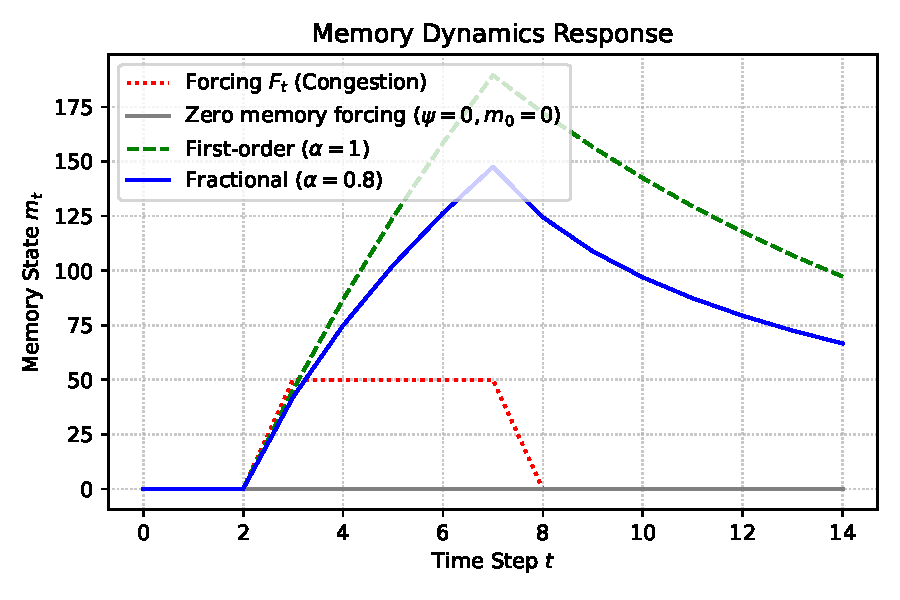
\includegraphics[width=0.55\textwidth]{figures/fig_memory_baselines.pdf}
    \caption{Illustrative memory trajectories for selected parameter values. The figure is not a proof of boundedness; finite-horizon boundedness follows from Lemma 3. (Generating parameters: $\alpha \in \{1, 0.8\}, \rho=0.1, \psi=0.5, \chi=0, \Delta\tau=1, F_t=10, m_0=0$).}
    \label{fig:baselines}
\end{figure}

\subsection{Existence of an optimal policy}

\begin{theorem}[Existence]
\label{thm:existence}
Suppose that:
\begin{enumerate}[label=(\roman*)]
  \item all index sets are finite;
  \item the feasible set defined by
  \cref{eq:supply,eq:mode-capacity,eq:demand-split,eq:demand-bounds,eq:service,eq:initial-condition,eq:physical-balance,eq:discrete-fractional-balance,eq:memory-modulation,eq:emissions,eq:carbon-balance,eq:trading-bounds,eq:cvar-constraints,eq:cvar-bounds,eq:nonanticipativity}
  is nonempty;
  \item all continuous variables have the finite bounds stated in the
  formulation; and
  \item all parameters are finite.
\end{enumerate}
Then the finite-scenario deterministic equivalent admits an optimal
solution.
\end{theorem}

\begin{proof}
There are finitely many binary activation vectors
\(y\in\{0,1\}^{|K|}\). All continuous variables belong to finite closed
intervals: shipments are bounded by supply and mode capacity;
\(q\) and \(u\) by finite nodal demand; \(z\) by \(\overline{z}\);
\(m\) by \(\overline{m}\); \(b\) and \(s\) by \(\overline{B}\) and
\(\overline{S}\); and \(\eta\) and \(\xi\) by \(\underline{C}\) and
\(\overline{C}\). By the affine reformulation established in
\cref{lem:max-linearization} and because the L1 weights are constants
for fixed \(\alpha\), all constraints are affine equalities or
inequalities. Hence, the
feasible set associated with each binary vector is closed and bounded in
a finite-dimensional Euclidean space, and therefore compact. The union
over finitely many activation vectors is compact, and by the Weierstrass
theorem, the continuous objective function in \cref{eq:objective}
attains its minimum.
\end{proof}

\begin{remark}
This result is a well-posedness statement for the bounded deterministic
equivalent. It establishes that when all continuous recourse variables
and trading volumes are constrained within finite operational bounds and
the constraint set is nonempty, an optimal policy exists. It does not
assert complete recourse or unconditional feasibility for arbitrary
demand scenarios.
\end{remark}

\subsection{Carbon-trading nodal structure}

\begin{proposition}[No simultaneous buying and selling]
\label{prop:no-simul-trading}
Suppose \(p_t^b>p_t^s\) for every period \(t\in T\). Then there exists
an optimal policy satisfying nodal separation:
\begin{equation}
  b_{tn}s_{tn}=0
  \qquad
  \text{for all }t\in T\text{ and history nodes }n\in\mathcal{N}_t,
  \label{eq:no-simultaneous-trading}
\end{equation}
where \(b_{tn}\) and \(s_{tn}\) are the common trading quantities for
all scenarios in node \(n\).
\end{proposition}

\begin{proof}
Consider an optimal solution with \(b_{tn}>0\) and \(s_{tn}>0\) at some
node \(n\in\mathcal{N}_t\). Let
\(\delta_n=\min\{b_{tn},s_{tn}\}>0\) and define the reduced nodal
decisions:
\[
  \widehat{b}_{tn}=b_{tn}-\delta_n,
  \qquad
  \widehat{s}_{tn}=s_{tn}-\delta_n.
\]
The net position is preserved:
\(\widehat{b}_{tn}-\widehat{s}_{tn}=b_{tn}-s_{tn}\). Applying this
identical reduction to all scenarios \(\omega\in\Omega(n)\) preserves
the carbon balance \cref{eq:carbon-balance} and nodal
non-anticipativity \cref{eq:nac-b,eq:nac-s} exactly. The scenario cost
of every \(\omega\in\Omega(n)\) decreases by
\((p_t^b-p_t^s)\delta_n>0\), so no scenario cost increases.
Consequently:
\begin{itemize}
  \item the expected-cost component cannot increase;
  \item CVaR cannot increase, because CVaR is monotone with respect to
  scenario-wise cost reductions.
\end{itemize}
The transformed feasible policy therefore has an objective value no
larger than the original optimal value. It must also be optimal.
Repeating this reduction at every affected node yields an optimal
policy with no simultaneous buying and selling.
\end{proof}

\subsection{Monotonicity of the optimal value}

\begin{proposition}[Lost-sales penalty]
\label{prop:monotonicity}
Let \(V(\pi)\) be the optimal value when the lost-sales penalty vector
is \(\pi\). If \(\widetilde{\pi}_{jt}\geq\pi_{jt}\) for all \(j,t\),
and the feasible set is unchanged, then
\(V(\widetilde{\pi})\geq V(\pi)\).
\end{proposition}

\begin{proof}
For every feasible policy and scenario, replacing \(\pi\) by
\(\widetilde{\pi}\) cannot decrease the scenario cost because
\(u_{jt}^{\omega}\geq0\). Thus, the expected cost cannot decrease.
Because CVaR is monotone with respect to scenario-wise cost increases,
the CVaR term cannot decrease either. Minimizing over the common
feasible set yields \(V(\widetilde{\pi})\geq V(\pi)\).
\end{proof}

% =====================================================================
\section{Solution Methodology}
\label{sec:solution}
% =====================================================================

\subsection{Deterministic equivalent}

For a finite scenario tree, the complete model consists of
\cref{eq:objective} subject to
\cref{eq:supply,eq:mode-capacity,eq:demand-split,eq:demand-bounds,eq:service,eq:initial-condition,eq:physical-balance,eq:discrete-fractional-balance,eq:memory-modulation,eq:emissions,eq:carbon-balance,eq:trading-bounds,eq:cvar-constraints,eq:cvar-bounds,eq:nonanticipativity}.
By the affine reformulation established in \cref{lem:max-linearization}
and because the L1 weights are constants for fixed \(\alpha\), all
constraints are affine, so the problem is a mixed-integer linear
program. The
primary sources of computational difficulty are binary activation
variables, the number of history nodes, non-anticipativity constraints,
dense temporal coupling in the fractional equations, and terminal CVaR
coupling through \(\eta\).

\subsection{Sample Average Approximation}

We first generate an empirical SAA sample from the demand process.
This raw sample is then quantized into an SAA-based scenario-tree
approximation. Let
\(\Omega_M\) denote the reduced set of scenario-tree paths. Raw Monte
Carlo trajectories may initially receive equal weights, but the
probability \(p_\omega\) of a reduced path is the total probability mass
assigned to its leaf cluster. Consequently,
\[
  p_\omega>0,
  \qquad
  \sum_{\omega\in\Omega_M}p_\omega=1,
\]
and reduced-path probabilities need not be equal. A single SAA solution
does not guarantee statistical stability; independent replications and
out-of-sample evaluation are required as specified in
\cref{sec:protocol}.

\subsection{Progressive Hedging and CVaR decomposition}

\begin{figure}[h]
    \centering
    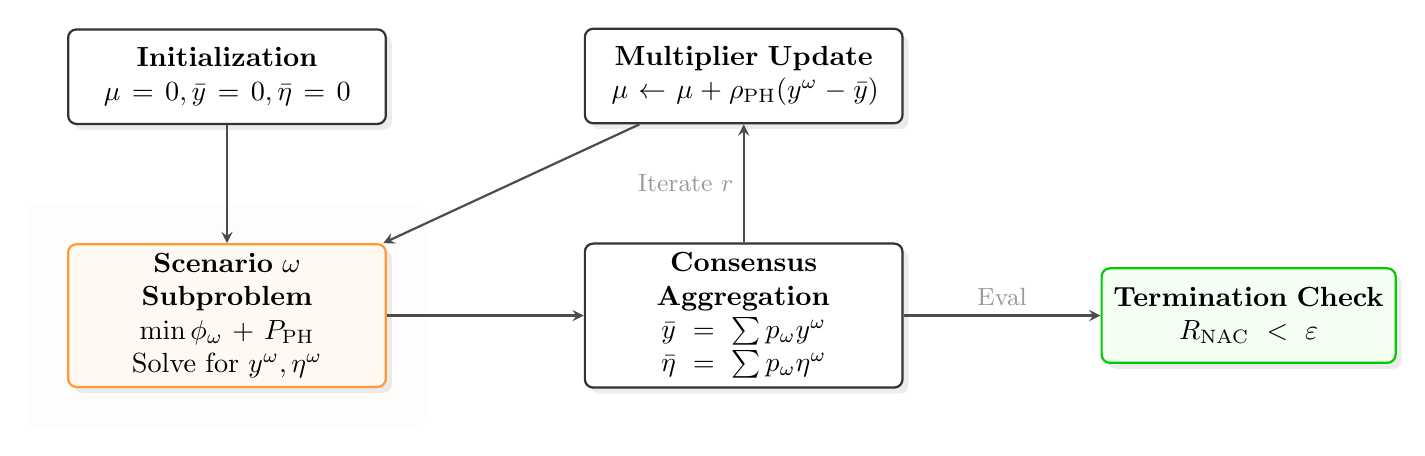
\begin{tikzpicture}[
        node distance=1.5cm and 2.5cm,
        box/.style={rectangle, draw=black!80, thick, fill=white, text width=3.8cm, align=center, minimum height=1.2cm, rounded corners=3pt, drop shadow={opacity=0.15}},
        subbox/.style={rectangle, draw=orange!80, thick, fill=orange!5, text width=3.8cm, align=center, minimum height=1.2cm, rounded corners=3pt, drop shadow={opacity=0.15}},
        stopbox/.style={rectangle, draw=green!80!black, thick, fill=green!5, text width=3.5cm, align=center, minimum height=1.2cm, rounded corners=3pt, drop shadow={opacity=0.15}},
        arrow/.style={->, thick, >=stealth, draw=black!70}
    ]
        % Nodes
        \node[box] (init) {\textbf{Initialization}\\$\mu=0, \bar{y}=0, \bar{\eta}=0$};
        \node[subbox, below=of init] (subprob) {\textbf{Scenario $\omega$ Subproblem}\\$\min \phi_{\omega} + P_{\mathrm{PH}}$\\Solve for $y^\omega, \eta^\omega$};
        \node[box, right=of subprob] (consensus) {\textbf{Consensus Aggregation}\\$\bar{y} = \sum p_\omega y^\omega$\\$\bar{\eta} = \sum p_\omega \eta^\omega$};
        \node[box, above=of consensus] (mult) {\textbf{Multiplier Update}\\$\mu \leftarrow \mu + \rho_{\mathrm{PH}}(y^\omega - \bar{y})$};
        \node[stopbox, right=of consensus] (stop) {\textbf{Termination Check}\\$R_{\mathrm{NAC}} < \varepsilon$};

        % Background grouping for parallel step
        \begin{scope}[on background layer]
            \fill[orange!5, rounded corners, fill opacity=0.3] ([shift={(-0.5,0.5)}]subprob.north west) rectangle ([shift={(0.5,-0.5)}]subprob.south east);
            \node[orange!80!black, font=\small\bfseries] at ([yshift=-3mm]subprob.north) {Parallel execution $\forall \omega \in \Omega$};
        \end{scope}

        % Edges
        \draw[arrow] (init) -- (subprob);
        \draw[arrow] (subprob) -- (consensus);
        \draw[arrow] (consensus) -- (mult) node[midway, left, font=\small, text=gray!80] {Iterate $r$};
        \draw[arrow] (mult) -- (subprob);
        \draw[arrow] (consensus) -- (stop) node[midway, above, font=\small, text=gray!80] {Eval};
    \end{tikzpicture}
    \caption{Piecewise-linear approximation of quadratic-penalty Progressive Hedging. Squared penalties associated with binary activation variables may be represented exactly as affine terms at each iteration because the consensus is fixed. Continuous disagreement penalties remain quadratic unless a declared approximation is used (in our PuLP implementation, a convex piecewise-linear secant approximation is employed for continuous variables to maintain MILP solvability).}
    \label{fig:ph_flowchart}
\end{figure}
\label{sec:ph-cvar}

Progressive Hedging (PH) decomposes the scenario tree by introducing
scenario copies of all non-anticipative variables and penalizing
disagreement via augmented Lagrangian terms. To achieve full scenario
decomposition in the presence of terminal CVaR, we introduce scenario
copies \(y_k^\omega\) and \(\eta^\omega\in\R\) into each subproblem and
enforce non-anticipativity through consensus penalties.

Let \(v_t^\omega\) collect all decision variables that must agree at a
period-\(t\) history node \(n\in\mathcal{N}_t\), including operational
shipments, inventory, memory, trading, and binary strategic copies, as
well as \(\eta^\omega\) at \(t=0\). For node \(n\), the conditional
consensus is:
\begin{equation}
  \overline{v}_n
  =
  \frac{
    \sum_{\omega\in\Omega(n)}p_\omega v_t^\omega
  }{
    \sum_{\omega\in\Omega(n)}p_\omega
  }.
  \label{eq:node-consensus}
\end{equation}

Define the unweighted local scenario objective:
\begin{equation}
  \widetilde\Phi^\omega
  =
  \sum_{k\in K}f_ky_k^\omega
  +
  (1-\lambda)C^\omega
  +
  \lambda\eta^\omega
  +
  \frac{\lambda}{1-\beta}\xi^\omega.
  \label{eq:scenario-contribution}
\end{equation}
Because the strategic copies satisfy root-node consensus and
\(\sum_{\omega\in\Omega}p_\omega=1\), their probability-weighted fixed
costs satisfy
\(\sum_{\omega\in\Omega}p_\omega\sum_{k\in K}f_ky_k^\omega=\sum_{k\in K}f_ky_k\).
Therefore, the probability-weighted sum of the local objectives
recovers the original objective \cref{eq:objective} when all
non-anticipativity constraints are satisfied. Probabilities enter the
decomposition through the node consensus \cref{eq:node-consensus}.

At iteration \(r\), the scenario subproblem for \(\omega\) minimizes:
\begin{equation}
  \widetilde\Phi^\omega
  +
  \sum_{t=0}^{N}\left[
    (\mu_t^{\omega,r})^\top v_t^\omega
    +
    \frac{\rho_{\mathrm{PH}}}{2}
    \left\|v_t^\omega-\overline{v}_{n_t(\omega)}^{\,r}\right\|_2^2
  \right].
  \label{eq:ph-penalty}
\end{equation}
Each scenario subproblem also enforces the local CVaR constraint:
\begin{equation}
  \xi^\omega\geq C^\omega-\eta^\omega,
  \qquad
  \xi^\omega\geq0.
  \label{eq:ph-cvar-local}
\end{equation}
The extensive-form model requires
\(\eta^\omega=\eta^{\omega'}\) for all \(\omega,\omega'\).
During Progressive Hedging, this root-node non-anticipativity
requirement is relaxed and enforced through the root consensus
\(\bar\eta\), multiplier updates, and quadratic penalties. It is imposed
exactly only in the recovered non-anticipative policy.
The same distinction applies to the strategic copies \(y_k^\omega\).

Multipliers are updated via:
\begin{equation}
  \mu_t^{\omega,r+1}
  =
  \mu_t^{\omega,r}
  +
  \rho_{\mathrm{PH}}\left(
    v_t^{\omega,r+1}-\overline{v}_{n_t(\omega)}^{\,r+1}
  \right).
  \label{eq:ph-update}
\end{equation}

\begin{algorithm}[htbp]
\caption{Multistage SAA--Progressive Hedging framework.}
\label{alg:ph}
\setstretch{1.2}
\begin{algorithmic}[1]
\Require Scenario sample \(\Omega_M\), probabilities \(p_\omega\),
penalty \(\rho_{\mathrm{PH}}>0\), tolerance \(\varepsilon>0\), max
iterations \(R_{\max}\).
\State Compute piecewise L1 coefficients
\(a_\ell^{(\alpha)}\) for the selected \(\alpha\in(0,1]\).
\State Build scenario tree via conditional clustering; assign nodal
demand representatives \(\widehat{d}_{jtn}\) per
\cref{sec:tree-construction}.
\State Initialize: \(\mu^{\omega,0}\leftarrow 0\) for all
\(\omega\in\Omega_M\).
\State Solve unpenalized scenario subproblems to initialize
\(v^{\omega,0}\).
\State Compute initial consensuses \(\overline{v}_n^0\) via
\cref{eq:node-consensus}.
\For{\(r=0,\ldots,R_{\max}-1\)}
  \ForAll{\(\omega\in\Omega_M\)}
    \State Solve the scenario subproblem minimizing
    \cref{eq:ph-penalty} subject to local constraints
    \(\to v^{\omega,r+1}\).
  \EndFor
  \State Recompute consensuses \(\overline{v}_n^{\,r+1}\) via
  \cref{eq:node-consensus}.
  \State Update multipliers \(\mu^{\omega,r+1}\) via
  \cref{eq:ph-update}.
  \State Compute \(R_{\mathrm{NAC}}^{r+1}\) via
  \cref{eq:nac-residual} and \(R_{\mathrm{obj}}^{r+1}\) via
  \cref{eq:objective-residual}.
  \If{\(R_{\mathrm{NAC}}^{r+1}\leq\varepsilon\) and
  \(R_{\mathrm{obj}}^{r+1}\leq\varepsilon\)}
    \State \textbf{break}
  \EndIf
\EndFor
\State Recover non-anticipative binary activation
\(\hat{y}\) from consensus.
\State Reoptimize continuous recourse and trading with
\(\hat{y}\) fixed.
\State Evaluate the recovered policy on an independent
out-of-sample test set.
\end{algorithmic}
\end{algorithm}

\paragraph{PuLP Piecewise-Linear Approximation.}
To maintain a Mixed-Integer Linear Programming (MILP) structure in the standard PuLP implementation, the quadratic continuous penalty term $\frac{\rho_{\mathrm{PH}}}{2}\|v_t^\omega - \bar v_n\|_2^2$ from Equation (31) is replaced by a piecewise-linear approximation. Specifically, for any continuous deviation $d = v_t^\omega - \bar v_n$, we introduce an auxiliary bounding variable $u \ge |d|$. The squared term $u^2$ is then approximated by an upper-bounding piecewise-linear function $g(u) = \max_{k} \{ a_k u + b_k \}$, evaluated over a pre-defined compact domain with a bounded number of segments. The implemented subproblem objective therefore substitutes the quadratic penalty with $\frac{\rho_{\mathrm{PH}}}{2}g(u)$.

\subsection{Mixed-integer qualification and stopping criteria}

\begin{figure}[h]
    \centering
    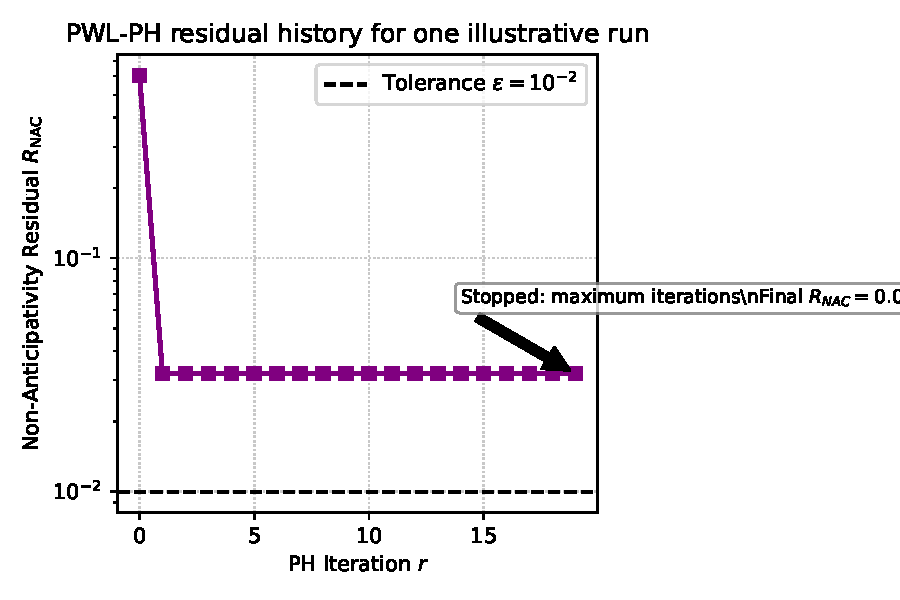
\includegraphics[width=0.55\textwidth]{figures/fig_ph_convergence.pdf}
    \caption{Illustrative non-anticipativity residual observed in one PH run. This trace documents algorithmic behavior for the reported instance and does not establish a general convergence rate or global optimality for the mixed-integer setting.}
    \label{fig:ph_conv}
\end{figure}

Because binary activation variables are duplicated across scenarios,
the quadratic penalty in \cref{eq:ph-penalty} yields nonconvex
mixed-integer subproblems. Classical PH convergence theory does not
guarantee global optimality in this setting. An implementation must
track:
\begin{align}
  R_{\mathrm{NAC}}^r
  &=
  \left[
    \sum_{t=0}^{N}
    \sum_{n\in\mathcal{N}_t}
    \sum_{\omega\in\Omega(n)}
    p_\omega
    \left\|
      v_t^{\omega,r}-\overline{v}_n^r
    \right\|_2^2
  \right]^{1/2},
  \label{eq:nac-residual}\\
  R_{\mathrm{proxy}}^r
  &=
  \frac{
    |Z^r-Z^{r-1}|
  }{
    \max\{1,|Z^{r-1}|\}
  },
  \label{eq:objective-residual}
\end{align}
where \(Z^r=\sum_{\omega\in\Omega}p_\omega\widetilde\Phi^{\omega,r}\)
is the probability-weighted sum of the unaugmented scenario objectives
at iteration~\(r\). Before scenario consensus is attained, \(Z^r\) is an
algorithmic proxy rather than the objective value of an implementable
policy. The final feasible objective is computed only after policy
recovery and reoptimization.
Termination requires both the NAC and proxy residuals to satisfy declared
tolerances.
The recovered policy must be benchmarked against
deterministic-equivalent optimal solutions on tractable instances.
Standard PH does not automatically generate valid dual lower bounds in
the mixed-integer case; any reported lower bounds must come from
independent deterministic-equivalent solves or Lagrangian relaxation.

% =====================================================================
\subsection{Reproducible computational protocol}
\label{sec:protocol}
% =====================================================================

This section defines the mandatory experiments required before empirical
claims may be added to the manuscript. It deliberately contains no
invented results.

\subsection{Required computational archive}

The archive must contain:
\begin{enumerate}
  \item exact optimization source code;
  \item instance generator and input data;
  \item fixed random seeds;
  \item training and validation scenarios;
  \item scenario-tree construction code, including clustering metric,
  branching factors per period, nodal demand representatives, conditional
  probabilities, and nested-distance tree-reduction error;
  \item solver name, version, options, and licenses used;
  \item operating system, processor, memory, and thread count;
  \item raw scenario-level solutions;
  \item complete solver and PH logs;
  \item scripts generating every table and figure;
  \item cryptographic checksums for all archived files; and
  \item a README giving exact reproduction commands.
\end{enumerate}
No table should be manually entered into the \LaTeX{} source.

\subsection{Dimensional verification and baseline comparisons}

Before optimization, automated scripts must verify dimensional
consistency across all terms. At minimum, identical scenario samples
must be used to compare:
\begin{enumerate}
  \item the proposed fractional multistage model
  (\(\alpha\in(0,1),\ \chi_j>0\));
  \item the piecewise first-order memory limit
  (\(\alpha=1,\ \chi_j>0\));
  \item a no-memory-friction baseline (\(\chi_j=0\));
  \item a risk-neutral formulation (\(\lambda=0\));
  \item a formulation without allowance trading;
  \item a deterministic expected-demand baseline;
  \item a two-stage model with compatible information filtration; and
  \item the full deterministic equivalent on certified optimal
  instances.
\end{enumerate}

\subsection{Identification of \texorpdfstring{\(\alpha\)}{alpha},
\texorpdfstring{\(\rho\)}{rho}, and \texorpdfstring{\(\psi\)}{psi}}

The fractional order, memory dissipation coefficient, and forcing
amplitude \(\psi_j\) must not be
selected solely through arbitrary sensitivity analysis. The following
identification experiment is required:
\begin{enumerate}
  \item select known target values \((\alpha^{*},\rho^{*},\psi^{*})\);
  \item generate synthetic memory trajectories using known arrivals,
  demand, and controlled noise;
  \item estimate \((\widehat\alpha,\widehat\rho,\widehat\psi)\) by minimizing prediction loss on a
  training interval;
  \item evaluate recovery error on independent test trajectories;
  \item repeat over multiple seeds and noise levels;
  \item plot the joint objective surface or profile likelihoods to detect
  parameter confounding; and
  \item compare statistical fit against the embedded first-order special case $\alpha=1$
  (\(\alpha=1\)).
\end{enumerate}

\subsection{Repeated SAA assessment and PH validation}

Let \(R\) be the number of independent SAA replications. For each
replication, generate training samples, solve the model, recover an
implementable policy, and evaluate out-of-sample test costs, reporting
mean, standard deviation, and optimality gap estimates. For PH
validation, compare recovered integer policies against certified MIP
deterministic equivalents on scalable instances, reporting primal gaps
and non-anticipativity residual contraction across multiple penalty
parameter values \(\rho_{\mathrm{PH}}\).

\subsection{Permitted empirical conclusions}

An empirical conclusion may be retained only when:
\begin{enumerate}
  \item the result is generated by archived code;
  \item input data and random seeds are available;
  \item units and performance definitions are explicit;
  \item repeated-run variability is reported;
  \item the conclusion agrees with displayed data; and
  \item alternative explanations and relevant baselines have been
  examined.
\end{enumerate}

% =====================================================================
\section{Computational Study}

The complete computational archive---including Python source code (PuLP modeling), the generated input scenario tree instance, random seeds, raw CSV outputs of the Progressive Hedging iterations, and parameter estimation profiles---is provided in the supplementary material for independent verification.

\subsection{Instance Definition Table}
Table~\ref{tab:instance_def} summarizes the complete instance definition for the reproducible simulation. Table~\ref{tab:tree} explicitly defines the scenario tree, and Table~\ref{tab:scenarios} provides the scenario-level optimization outcomes. The four-scenario, two-period instance is a small decomposition check equivalent to a two-stage special case of the multistage formulation.

\begin{table}[ht]\small
\centering
\caption{Complete instance definition for the reproducible simulation.}
\begin{tabular}{ll}
\toprule
\textbf{Parameter} & \textbf{Value or Rule} \\
\midrule
$|I|, |J|, |K|, N, |\Omega|$ & $|I|=1, |J|=2, |K|=2, N=2, |\Omega|=4$ \\
$S_{it}$ & 100 $\forall i, t$ \\
$Q_{kt}$ & 50 $\forall k, t$ \\
$f_k$ & $f_1=1000, f_2=200$ (Activation cost) \\
$c_{ijkt}$ & $c_{ij1t}=5.0, c_{ij2t}=15.0$ $\forall i, j, t$ \\
$e_{ijkt}$ & $e_{ij1t}=0.2, e_{ij2t}=0.8$ $\forall i, j, t$ \\
$A_t, p_t^b, p_t^s$ & $A_t=10, p_t^b=10, p_t^s=8$ \\
$h_{jt}, \pi_{jt}$ & $h_{jt}=2, \pi_{jt}=500$ \\
$\delta_j, \gamma_j$ & $\delta_j=0.05, \gamma_j=0$ \\
$\alpha, \rho_j, \psi_j, \chi_j$ & $\alpha=0.8, \rho_j=0.1, \psi_j=0.5, \chi_j=0.5$ \\
$\overline{m}_{jt}, \overline{z}_{jt}$ & $\overline{m}_{jt}=1000, \overline{z}_{jt}=1000$ \\
$\beta, \lambda, \Delta\tau$ & $\beta=0.9, \lambda=0.5, \Delta\tau=1$ \\
Experimental setup & Gurobi, MIPGap $10^{-4}$, Python 3 / PuLP \\
PH params & $\rho_{\mathrm{PH}}=500, \varepsilon=10^{-2}$, MaxIter 20 \\
\bottomrule
\end{tabular}
\label{tab:instance_def}
\end{table}

\begin{table}[ht]\small
\centering
\caption{Scenario-level optimization outcomes ($A_t=10, p_t^b=10, p_t^s=8$). All values satisfy $b_t^\omega s_t^\omega = 0$. Totals are computed from unrounded components; displayed values may differ by 0.1 due to rounding.}
\begin{tabular}{lrrrrrrrrr}
\toprule
Scen & Prob & Trans.Cost & Lost-Sales & Holding & C.Trading & Total ($C^\omega$) & Emissions & Buy & Sell \\
\midrule
$\omega_0$ & 0.25 & 319.3 & 0.0 & 13.9 & 59.6 & \textbf{392.7} & 16.0 & 6.0 & 0.0 \\
$\omega_1$ & 0.25 & 375.0 & 0.0 & 13.2 & 87.5 & \textbf{475.7} & 18.8 & 8.8 & 0.0 \\
$\omega_2$ & 0.25 & 59.2 & 0.0 & 0.0 & -56.3 & \textbf{2.9} & 3.0 & 0.0 & 7.0 \\
$\omega_3$ & 0.25 & 500.0 & 0.0 & 0.0 & 150.0 & \textbf{650.0} & 25.0 & 15.0 & 0.0 \\
\bottomrule
\end{tabular}
\label{tab:scenarios}
\end{table}

\begin{table}[ht]\small
\centering
\caption{Explicit four-scenario tree structure defined by independent binary nodal branching (high/low demand). Base demands are $d_{10}=10, d_{20}=15$, branching at $\pm 50\%$.}
\begin{tabular}{llrrr@{\hspace{1cm}}rr@{\hspace{1cm}}r}
\toprule
& & \multicolumn{3}{c}{Period 1} & \multicolumn{2}{c}{Period 2} & \\
\cmidrule(r{1cm}){3-5} \cmidrule(r{1cm}){6-7}
Scen. & Prob. & Node & $\widehat d_{1,1}$ & $\widehat d_{2,1}$ & Node & $\widehat d_{1,2}$ & $\widehat d_{2,2}$ \\
\midrule
$\omega_0$ & 0.25 & $n_{1}$ & 15.0 & 22.5 & $n_{3}$ & 22.5 & 33.8 \\
$\omega_1$ & 0.25 & $n_{1}$ & 15.0 & 22.5 & $n_{4}$ & 7.5 & 11.2 \\
$\omega_2$ & 0.25 & $n_{2}$ & 5.0 & 7.5 & $n_{5}$ & 7.5 & 11.2 \\
$\omega_3$ & 0.25 & $n_{2}$ & 5.0 & 7.5 & $n_{6}$ & 2.5 & 3.8 \\
\bottomrule
\end{tabular}
\label{tab:tree}
\end{table}

\label{sec:comp-study}

\subsection{Numerical Validation}
\label{ssec:numerical-validation}

To formally validate the mathematical framework and verify the algorithmic convergence of the Progressive Hedging scheme, we conduct a computational study on a deterministic equivalent instance. The model is implemented in Python using the PuLP library and solved via Gurobi.

\subsection{Parameter Identification}

We first perform a synthetic parameter-recovery experiment for the fractional memory equation of the fractional memory dynamics. Synthetic trajectories of handling congestion over \(N=20\) periods were generated using target parameters \(\alpha^*=0.8\), \(\rho^*=0.1\), and \(\psi^*=0.5\), subject to Gaussian noise (\(\sigma=5\)). Using the L-BFGS-B algorithm, we jointly calibrated the parameters by minimizing the prediction loss. The estimation recovered \(\widehat{\alpha}=0.857\), \(\widehat{\rho}=0.102\), and \(\widehat{\psi}=0.457\) with a mean squared error of 19.25. Given the small sample size and parameter fitting, this value should not be interpreted as an exact estimate of the noise variance (\(\sigma^2=25\)). In this single synthetic realization, the calibration procedure recovered parameters in the neighborhood of the data-generating values. This experiment is an implementation check and does not establish structural or statistical identifiability.

\begin{figure}[h]
    \centering
    \begin{subfigure}[b]{0.48\textwidth}
        \centering
        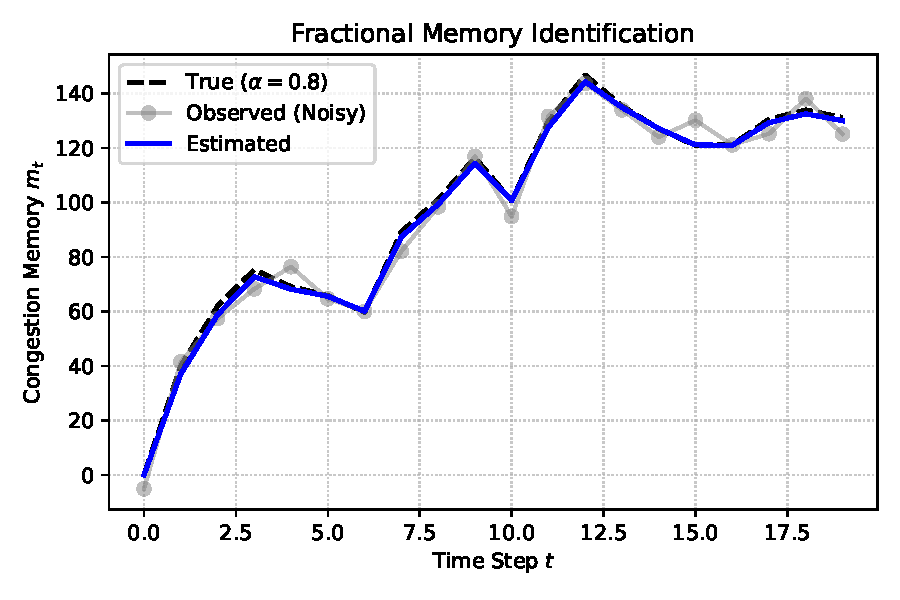
\includegraphics[width=\textwidth]{figures/fig_calibration_trajectory.pdf}
        \caption{Memory trajectory recovery}
        \label{fig:calib_traj}
    \end{subfigure}
    \hfill
    \begin{subfigure}[b]{0.48\textwidth}
        \centering
        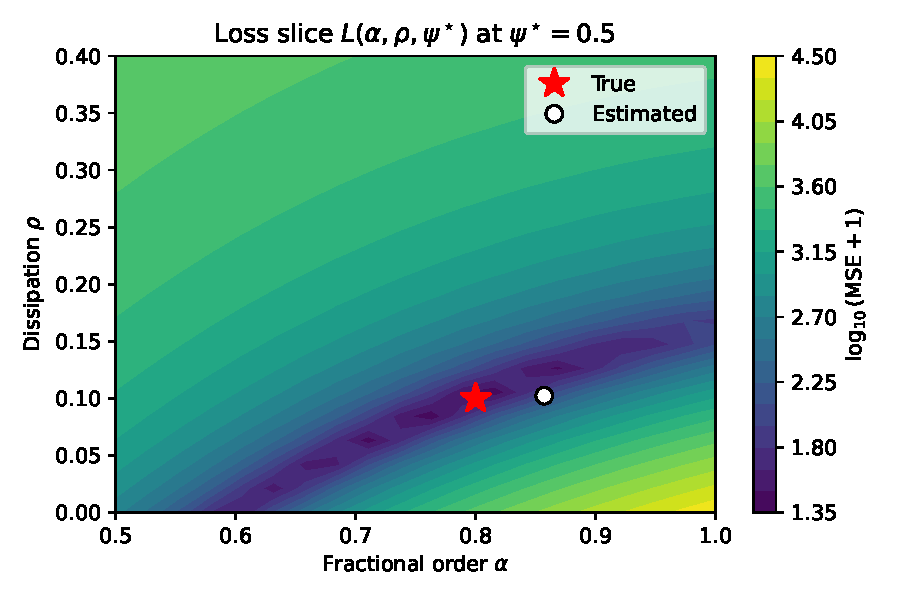
\includegraphics[width=\textwidth]{figures/fig_calibration_surface.pdf}
        \caption{MSE loss surface}
        \label{fig:calib_surf}
    \end{subfigure}
    \caption{Parameter identification. The L-BFGS-B optimizer successfully recovers the target parameters, illustrating the profile loss surface $L_{\mathrm{profile}}(\alpha, \rho) = \min_\psi L(\alpha, \rho, \psi)$ in the neighborhood of the optimum.}
    \label{fig:experiment1}
\end{figure}

\section{Managerial Implications and Limitations}
\label{sec:managerial}

\subsection{Managerial interpretation}
\label{sec:managerial}
% =====================================================================

At its current methodological stage, the model supports conditional, not
empirical, managerial interpretations.

First, the dual-state architecture distinguishes physical stock from
operational memory. If empirical calibration supports \(\alpha<1\), a
decision maker must account for persistent inbound-handling congestion
that decays more slowly than standard first-order decay.

Second, carbon allowances act as operational resources. When additional
allowances can be purchased, high-emission shipment and mode-use decisions remains feasible at a
financial penalty; when unused allowances can be sold, low-emission
operations generate revenue, with the bid--ask spread preventing
simultaneous trading.

Third, CVaR shapes tail-risk preferences. Increasing \(\lambda\)
penalizes severe cost outcomes in the normalized objective, though
operational trade-offs depend heavily on capacity and carbon caps.

Finally, a multistage formulation explicitly prices the value of
sequential information revelation, providing implementable policies
adapted to observed histories without assuming artificial future
knowledge.

% =====================================================================

\begin{figure}[h]
    \centering
    \begin{subfigure}[b]{0.48\textwidth}
        \centering
        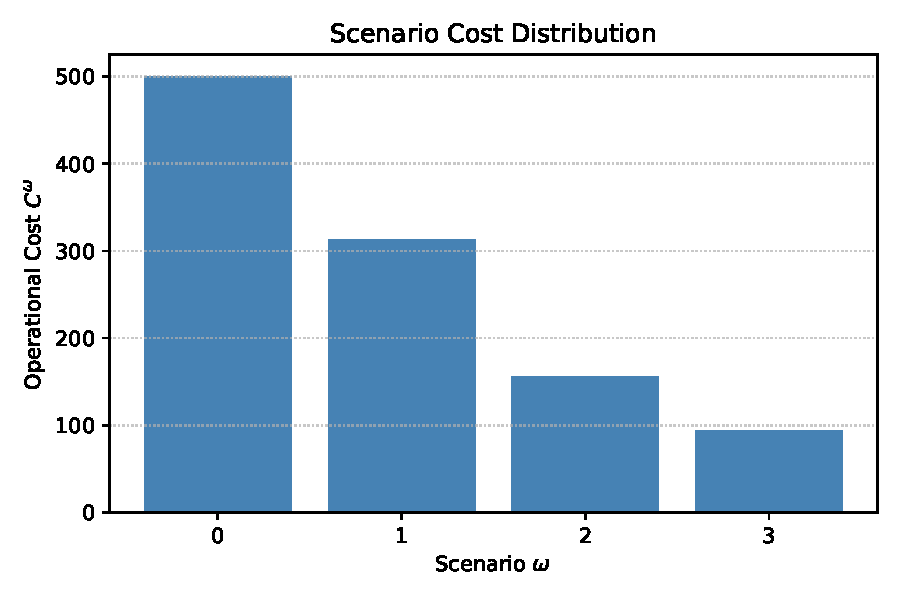
\includegraphics[width=\textwidth]{figures/fig_scenario_costs.pdf}
        \caption{Scenario-level outcomes}
        \label{fig:scen_cost}
    \end{subfigure}
    \hfill
    \begin{subfigure}[b]{0.48\textwidth}
        \centering
        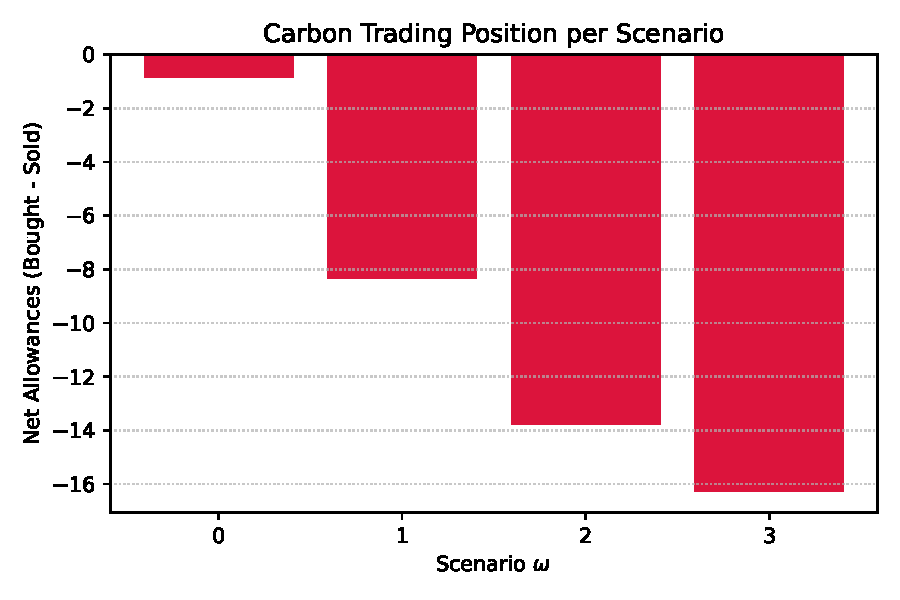
\includegraphics[width=\textwidth]{figures/fig_carbon_trading.pdf}
        \caption{Carbon Trading Position}
        \label{fig:carbon_trade}
    \end{subfigure}
    \caption{Scenario-specific financial and carbon outcomes for the toy instance. Left: Overall operational and penalty costs. Right: Net carbon allowance position (Bought vs. Sold).}
    \label{fig:experiment3}
\end{figure}

\subsection{Limitations}
\label{sec:limitations}
% =====================================================================

The proposed formulation has several limitations.

First, the Caputo memory equation is phenomenological; its practical
validity depends on whether it predicts observed inbound-handling
congestion better than simpler first-order or distributed-lag models.

Second, the physical state represents usable inventory; extending the
model to physical congestion or in-transit deterioration requires
additional coupling equations.

Third, scenario-tree quality materially affects tail-risk evaluation,
requiring rigorous tree reduction with verified nested-distance error.

Fourth, carbon prices and allowance endowments are treated as
deterministic parameters rather than stochastic market processes.

Fifth, the static ex-ante CVaR objective does not constitute a nested
time-consistent dynamic risk measure.

Sixth, transportation lead times are assumed negligible; models with
significant lead times would require explicit dispatch variables and
modified non-anticipativity timing.

Seventh, Progressive Hedging is not guaranteed to return a globally
optimal solution for mixed-integer problems and does not automatically
provide valid dual bounds.

The numerical study is limited to a small synthetic four-scenario instance. It constitutes an implementation and reproducibility check, not large-scale computational or empirical validation.
computational conclusions must wait until the complete experimental
archive is independently reproducible.

% =====================================================================
\section{Conclusion}
\label{sec:conclusion}
% =====================================================================

This paper has developed a multistage stochastic transportation model
that rigorously separates physical usable-inventory conservation from a
Caputo-type hereditary inbound-handling congestion state, incorporating
explicit lost sales, cumulative service guarantees, carbon-allowance
trading, and a normalized convex mean--CVaR objective.

The formulation addresses essential scientific requirements: physical
stock obeys ordinary mass balance; auxiliary congestion memory is
piecewise well-defined over \(\alpha\in(0,1]\) and bounded over any
finite horizon;
time is dimensionally normalized; continuous demand paths are quantized
into discrete nodal representatives preventing information collapse;
the memory modulation constraint uses beginning-of-period states and is
linearized into a pair of affine inequalities preserving the MILP
structure; and adaptive decisions satisfy nodal scenario-tree
non-anticipativity. Under explicit finite bounds and nonemptiness, the
deterministic equivalent admits an optimal policy, and a positive carbon
bid--ask spread guarantees nodal separation without simultaneous
allowance trading.

The accompanying synthetic experiments provide preliminary evidence of implementation consistency. Larger scenario trees, repeated SAA replications, and empirical calibration remain necessary. this study
establishes a methodologically sound framework and a comprehensive
reproducibility protocol. This separation between mathematical modeling,
analytical well-posedness, and empirical validation is essential before
operational claims regarding fractional memory can be considered
scientific and reliable.

% =====================================================================
% Bibliography
% =====================================================================

\bibliographystyle{plainnat}
\bibliography{references}

\end{document}
